\documentclass[a4paper]{article}

% Font tiếng Việt
\usepackage[T5]{fontenc}
\usepackage[utf8]{inputenc}
\DeclareTextSymbolDefault{\DH}{T1}

% Tài liệu tham khảo
\usepackage[sorting=nty,backend=bibtex,defernumbers=true,maxbibnames=99]{biblatex}
\usepackage{url} % long URL
\usepackage[unicode]{hyperref} % Bookmark tiếng Việt
\usepackage{graphicx}
%Đổi tên mặc định
\renewcommand{\contentsname}{Mục lục}

\addbibresource{reference.bib}


\begin{document}

%Tiêu đề
\title{CTT405\\
Báo cáo cuối kỳ\\[1cm]
Combining Natural Logic and Shallow Reasoning for Question Answering
}
\author{Vũ Ngọc Minh Hoàng - 1412186
Bùi Quốc Bảo - }
\maketitle

%Số trang
\pagenumbering{roman}
%\setcounter{page}{1}

%Mục lục
\tableofcontents
\pagenumbering{arabic}

\clearpage

\section{Tổng quan}
%Phát biểu bài toán, input output là gì?
Bài toán của chúng ta phát biểu như sau:
\begin{enumerate}
\item Cho một bộ dữ liệu lớn để làm knownledge base
\item Dữ liệu dùng để đánh giá là các câu hỏi có nhiều lựa chọn
\item Nhiệm vụ của máy là tìm dẫn chứng từ knownledge base để tìm xem lựa chọn nào phù hợp
\end{enumerate}
Có khá nhiều cách để máy xác định lựa chọn, trong đó có phương pháp Combining Natural Logic and Shallow Reasoning sẽ được giới thiệu kĩ ở các phần sau.


%Tại sao cần giải bài toán này? 
Phương pháp được giới thiệu sau đây đóng góp rất lớn cho việc tìm kiếm thông tin hoặc trích xuất thông tin trong một cơ sở tri thức.
%Các ứng dụng/ cần thiết của bài toán?

Bài toán của chúng ta khá giống với bài thi Reading trong IELTS. Chúng ta sẽ được đưa cho nhiều mệnh đề và phải dựa vào bài đọc để xác định xem mệnh đề đó thuộc nhãn TRUE, FALSE hay NOT GIVEN.
\section{Các công trình liên quan}
%Có những hướng giải quyết bài toán như thế nào?
%Tóm tắt các phương pháp đã được thực hiện trước đó
%Ưu nhược của các phương pháp trước (đã được tác giả tóm tắt/bạn biết được)

\section{Phương pháp}
%Trình bày chi tiết phương pháp giải quyết bài toán trong paper.

\section{Thực nghiệm và kết quả}

%Dữ liệu
Đánh giá dựa trên bộ dữ liệu SCITEXT. Gồm các câu hỏi khoa học dành cho học sinh lớp 4. Quá trình train sẽ tạo ra cây quan hệ như ở phần NaturalLI đã giới thiệu bằng các câu câu trả lời đã được gán nhãn, ở phần test sẽ chỉ đưa các câu hỏi vào cây để tìm ra câu support cho nó.
%Thực hiện thực nghiệm

\subsection*{Đặt vấn đề}
Lấy ví dụ về trường hợp sau:
\begin{itemize} 
\item[] P: Food serves mainly for growth, energy and body repair, maintenance and protection. 
\item[] H: Animals get energy for growth and repair from food. 
\end{itemize}
Từ 2 câu trên ta thấy được form của chúng như sau:

Food serves mainly for x -> Animals get x from food

Mặc dù có đủ thông tin nhưng NaturalLI sẽ không tìm thấy câu support. Vì lý do đó, chúng ta cần một đánh giá để xác định độ tốt của thuật toán.

\subsection*{Đánh giá độc lập các keyphrase}
Chúng ta sẽ đánh giá độc lập các keyphrase, phương pháp này gồm 2 bước là xác định keyphrase và match giữa 2 câu.
Keypharse là một cụm từ trong câu, có thể xác định thông qua các cách như sau:
\begin{itemize} 

\item[•]	một danh từ, có thể có tính từ phía trước hoặc được nối giữa of và sở hữu ‘s
.sneaky kitten or pail of water
\item[•]	một động từ, có thể có trạng từ phía trước
.e.g., quietly pounce
\item[•]	một danh từ có danh động từ phía trước
.flowing water 
\item[•]	Động từ to be sẽ không làm một keyphrase
\end{itemize}
Sau khi đã xác định các keyphrase, ta sẽ match các keyphrase ở 2 câu như sau:
\begin{enumerate}
\item Đầu tiên, tất cả các keyphrase giống nhau sẽ được nối với nhau. 
(stove, transferred)
\item Sau đó, các keyphrase có hậu tố và tiền tố giống nhau sẽ được nối với nhau.
(suffix: heat energy – thermal energy)
\item Nếu keypharse này cũng chứa keyphrase kia thì cũng sẽ được nối
(heat water – water)
\item Cuối cùng, các keyphrase bị “kẹp” giữa 2 keyphrase được nối khác thì cũng sẽ được nối.
\end{enumerate}
Ví dụ như trường hợp sau:
\begin{center}
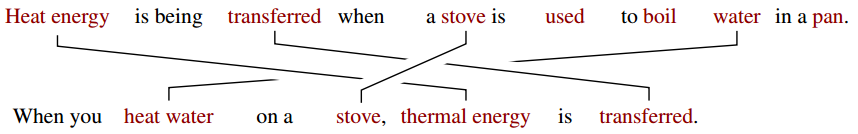
\includegraphics[scale=0.5]{vidu}

\end{center}
Sự tương đồng giữa 2 câu sẽ được tính thông qua một số điểm được tính bằng công cụ Solr. Số điểm này sẽ dựa trên số cặp keyphrase được nối, số cặp keypharse được match chính xác với nhau và số keyphrase không được nối.

\subsection*{Một đánh giá khác}
\begin{itemize} 
\item[] P: some cats have tails 
\item[] H: no cats have tails
\end{itemize}
Ta có thể thấy 2 câu trên có ý đối lập hoàn toàn với nhau, ta cũng sẽ xét sự đối lập của nó.
2 câu được xem là phù hợp với nhau nếu:
\begin{itemize}
\item[•] Chúng có cùng “lemmatized” (có cùng gốc từ)
\item[•] Chúng giống nhau về “polarity” 
\end{itemize}
%Kết quả và bàn luận kết quả?

\begin{table}[!th]
\begin{center}
\begin{tabular}{|l|c|r|}
\hline
System & Train & Test \\
NaturalLI & 65\% & 61\% \\
NaturalLI cải tiến & 74\% & 67\% \\
\hline
\end{tabular}
\end{center}
\caption{Kết quả thực nghiệm}
\label{ex:table}
\end{table}

Phương pháp đã cải thiện lên hơn 5\%.
Thông qua phương pháp này, chúng ta nhận ra rằng:
\begin{itemize}
\item[•] Áp dụng suy luận vào dependency tree,
\item[•] Sử dụng soft evaluation function để tìm ra các lựa chọn gần đúng
\item[•] Cuối cùng, chứng tỏ rằng có thể sử dụng relational entailment và meronymy để hỗ trợ cho natural logic.
\end{itemize}
%Ví dụ tham khảo tài liệu
This document is an example of BibTeX using in bibliography management. Three items 
are cited: \textit{The \LaTeX\ Companion} book \cite{latexcompanion}, the Einstein
journal paper \cite{einstein}, and the Donald Knuth's website \cite{knuthwebsite}. 
The \LaTeX\ related items are \cite{latexcompanion,knuthwebsite}. 

\clearpage

% In tài liệu tham khảo
\addcontentsline{toc}{section}{Tài liệu tham khảo}
\printbibliography[heading=subbibliography, title={Tài liệu tham khảo}]

\end{document}